% This is samplepaper.tex, a sample chapter demonstrating the
% LLNCS macro package for Springer Computer Science proceedings;
% Version 2.21 of 2022/01/12
%
\documentclass[runningheads]{llncs}
%
\usepackage[T1]{fontenc}
% T1 fonts will be used to generate the final print and online PDFs,
% so please use T1 fonts in your manuscript whenever possible.
% Other font encondings may result in incorrect characters.
%
\usepackage{graphicx}
% Used for displaying a sample figure. If possible, figure files should
% be included in EPS format.
%
% If you use the hyperref package, please uncomment the following two lines
% to display URLs in blue roman font according to Springer's eBook style:
%\usepackage{color}
%\renewcommand\UrlFont{\color{blue}\rmfamily}
%\urlstyle{rm}
%

\begin{document}
%
\title{An Expert System for Real Estate Recommendations}
%
%\titlerunning{Abbreviated paper title}
% If the paper title is too long for the running head, you can set
% an abbreviated paper title here
%
\author{José Coelho\inst{1} \and Luciano Dias\inst{2}
\and Joana Vaz\inst{2} \and Miguel Rodrigues \inst{3} \and Luís Paula \inst{4}}

\institute{University of Madeira, Funchal, PT \and Instituto Superior de Engenharia do Porto, Porto, PT \and Instituto Superior Politécnico de GAYA, VN Gaia, PT \and Universidade do Minho, Braga, PT}
%
\maketitle              % typeset the header of the contribution
%
\begin{abstract}
Finding and purchasing a real estate property can be a delicate and challenging process due to the inherent influence of different factors. Even though there's been a lot of work done in the real estate recommendation space, most systems still lack accessibility and focus on user preference. Advanced AI applications and features are still being developed and are usually too expensive for the average property buyer. This paper describes the design and implementation of an expert system designed to provide recommendations for real estate properties for potential buyers with a focus on the user experience and preferences by incorporating a user friendly application that offers a good user-experience. Results demonstrate the systems potential as an early stage prototype, showing an ability to align recommendations to user individual needs. This approach proposes a scalable solution that could improve the usability for both final buyers and real estate agents.

\keywords{Expert Systems  \and Real Estate \and Artificial Intelligence.}
\end{abstract}
%
%
%
\section{Introduction}

Expert systems are computer applications designed to mimic the human expertise in its area of application. This is achieved by, among other things, applying logical inference and rule-based reasoning over the domain knowledge.

Created in the 70s and 80s, it was regarded by many as the first truly successful Artificial Intelligence application. Three crucial components are required to make these systems a success: an inference engine, a knowledge base and an expert willing to encode their knowledge into these systems.
These systems brought light to the importance of being able to represent t well structured domain knowledge and data. ultimately influencing the rise of subjects of study such as \textit{Machine Learning} and neural networks where data and its correctness are considered a crucial component to these newer systems.

Expert systems applications have been divided into 10 categories\cite{hayesroth}. Interpretation, Prediction, Diagnosis, Design, Planning, Monitoring, Debugging, Repair, Instruction and Control. In this article we describe an Interpretation expert system, designed to make sense of domain knowledge by categorizing or labeling input according to predefined rules. This system interprets various real estate property attributes - like security, accessibility and energy efficiency - to determine its suitability for potential buyers.

It does this by trying to assign value - which we call the property score - to each property it analyzes. It is well established that there is intrinsic value in real estate properties, however with this system, more than anything, it tries to determine the value of the property to the user. The final goal is to make the user happy.

\section{State of the Art}

\subsection{Property evaluation techniques}
\subsubsection{Traditional Techniques}
\paragraph{}
Pagourtzi E. et al.\cite{methods} describes traditional techniques as those that are performed through direct comparison of capital or by determining a regression model based on a range of observations. These might include the following methods:
\begin{itemize}
    \item Comparable method
    \item Profits method
    \item Investment/income method
\end{itemize}

These methods tend to focus on the monetary value the property is assigned by the market or the value other similar properties were assigned.
The investment/income method is a method of simple comparison, it takes into account the investment the property is estimated to need and the income the property is expected to produce, doing so by looking at the transactional history of similar properties in the same area. The profit method, on the other hand, takes a business focus approach by trying to determine the profit that a business might be able to achieve with the property being evaluated.

The expert system detailed in this paper is designed not only on the inherent value of a property but also the preferences that the user might have that can also be attributed to the property under evaluation.

\subsubsection{Advanced Techniques}
\paragraph{}
More advanced methods have been developed and these try to model and emulate the actions and thought processes of the actors in the market. These are considered more quantitative methods \cite{methods}. These could be methods such as:
\begin{itemize}
    \item Artificial neural networks (ANNs)
    \item Fuzzy logic methods
    \item spatial analysis methods
\end{itemize}

These methods are what we would more closely consider today as being Artificial Intelligence methods. ANNs, for example, can be trained from the extensive amount of data about the real estate market to predict or interpret the value of a real estate property.

Spatial analysis, as the name suggest, try to determine the value of properties based on their location and relationships found in data concerning those locations.

Determining the value of a property is not an exact science most of the time, it is very nuanced, that's why \textbf{fuzzy logic} has been used in such methods. It favors linguistic variables over numbers which might make sense when the system's focus is on the user and their preferences.

\subsection{Automated Valuation Models (AVMs)}

On of the most common systems for evaluating real estate properties market value is Automated Valuation Models - or AVMs for short. These models leverage mathematical modeling techniques, in an automated manner, in order to generate property valuations quickly and, ideally, accurately. Such techniques include data sources, statistical models and machine learning algorithms.

AVMs analyze a variety of data in order to produce their estimation, including:
\begin{itemize}
    \item Historical sales data - previous prices of comparable properties
    \item Market trends - macroeconomic data, such as interest rates and housing market trends
    \item Asking prices - current asking prices in the property's market
    \item Property attributes - the attributes of the property being evaluated
    \item Transactional data - house market transactions
\end{itemize}

The expert system described in this article uses both the Property attributes and the asking price to compare and evaluate properties.

\subsubsection{Disadvantages}
\paragraph{}
A big disadvantage of this system is that, usually, it does not take into account the actual physical condition of the property. Instead an average condition is assumed which may not always be the case.

Some of these models use transactional data, this can sometimes reveal problematic as the recency of this data might not be the most appropriate and might make the system overlook the current state of the market.

\subsection{Machine Learning and Data-Driven models}

Machine learning and other data driven models have been gaining traction among applications that need to learn from data.
Given the amount of data that this domain, ie. real estate valuation, requires it's only natural that this too is a perfect use case for machine learning applications.

Some authors, for example, have used machine learning to develop housing price prediction models, as is the case of Park and Bae\cite{bpark} and Baldominos et al.\cite{mlinrealestate}. These applications focus specifically on predicting property prices taking into account, among other things, property attributes. The expert system in this article focuses on determining the suitability of a property to a client, using this same data.

Oh and Tan\cite{reinforcement} demonstrated that it was possible to use reinforcement learning - an interdisciplinary area of Machine Learning - to develop agents that could aid users in identifying properties they might be interested in, making better recommendations that other systems that propose to do the same.

\subsection{Expert Systems in Real Estate}

There is effectively a lot of prior work on using Expert Systems for many different applications in the Real Estate domain. Hossein et al.\cite{hossein} designed and implemented a fuzzy Expert System to provide recommendations of real estate properties. This cover exactly the same use case that this paper's expert system is being applied to.

The authors of the previously mention paper have concluded, with user testing and surveys, that compared to conventional real estate systems, the expert system they developed was much less time consuming for users. They were also able to determine that this expert system could in fact be a replacement for a human expert in some situations.

\subsection{Limitations in Current Systems}

As discussed previously there has been an abundance of prior work done, and there are a lot of applications, mostly web applications, that cater to such use cases. This comes to no surprise given that real estate is a significant sector of the global economy which moves a lot of capital. As an example, according the Banco de Portugal (Bank of Portugal)\cite{bancoportugal} in September 2024 the total amount of bank loans extended to individuals for home purchases rose to over two thousand and seven hundred million euros. This shows a clear incentive for private initiatives to develop such systems that can help users find the best deals they can.

Though the systems currently in place for real estate recommendations are powerful, they remain static through time and haven't seen real implementation of Artificial Intelligence applications to help users.

Browsing through three of the top real estate portals in Portugal - idealista.pt, imovirtual.pt and supercasa.pt - we can quickly confirm that there is still no AI features. The user journey takes the classic form of the user initiating the interaction and going through all the steps of searching, filtering and picking the properties that are most adequate to what they are looking for.

Our expert system hopes to change that and influence future work on this domain.

\section{Methodology}

\subsection{Data Collection and Processing}

For most intelligent systems data is a crucial part of its workings. Some systems are only as good as their data, and it has become clear in recent years that data correctness and availability is a tenet of artificial intelligence applications.

For this expert system we had to gather and handle data so that we could feed it to our system, we implemented a ETL methodology - Extract, Transform and Load.

\subsubsection{Extract}
Firstly, we developed a python script to scrape one of the biggest websites for real estate property advertising and store that data on disk so that it could be processed later.

Once we had the data we made a visual and manual run through of the data and noticed a few problems with it.
\begin{itemize}
    \item Some properties were missing some attributes,
    \item Some attributes were using the wrong data type, for example the price as a string instead of a float
    \item Some string attributes had special characters that had to be removed
\end{itemize}

\subsubsection{Transform}
Given the amount of data we collected (around 600 properties) we implemented another python script to automatically detect and correct the situations reported above. This tasks was crucial as data correctness is extremely important to obtain correct results.

Another important aspect of data handling is the format the data is in. Having the data in a format that is easy to read and process both by humans as well as computers is crucial. Hence we transformed the data into the JSON format so that it could be easily processed and understood.

\subsubsection{Load}
Now that we have correct and predictable data it was time to feed it to our system. For the Prolog system implementation we had to develop a python script that loaded the JSON data and converted it to Prolog facts. For the Drools implementation, since it's based on the Java language, a higher level language, it was easier to load and import the data with Java itself.

\subsection{System Architecture}

One of the most important aspects of the expert system we developed was to provide a good User Experience and to help the user reach its goals. Therefore we decided that we would expose the expert system through a Web application so that we could present users with a clean and intuitive user experience and interface.

The web application is composed of several components:
\begin{enumerate}
    \item a Prolog inference engine
    \item a Prolog HTTP server
    \item a proxy Web API
    \item a Drools engine and HTTP server
    \item a front-end application
    \item python utilities to process data
\end{enumerate}

\begin{figure}
    \centering
    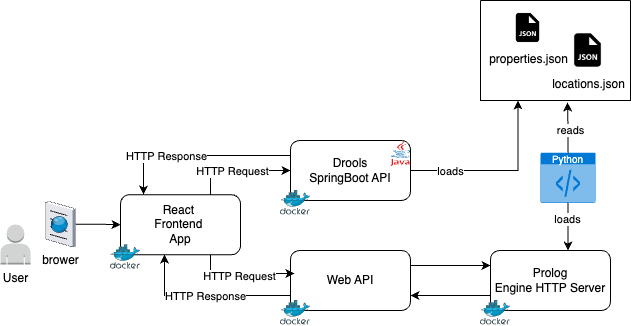
\includegraphics[width=0.9\linewidth]{expert-system.drawio.png}
    \caption{High level overview of the system architecture}
    \label{fig:system-architecture}
\end{figure}

The Prolog inference engine is responsible for interpreting the domain knowledge and infer and extract the conclusions we'd like to show to our users. In order to expose this information we implemented an HTTP server in Prolog, however the data structure that this component serves was not the most appropriate so we decided to add another layer, a proxy Web API.

The proxy Web API is responsible for providing a simple and standard interface between the Prolog engine and the front-end application, or any other clients. This Web API gets HTTP requests from clients (eg. the front-end application), transforms that request into a request that Prolog can understand and then forwards that request to Prolog. The Prolog HTTP server processes the request and sends back a response to the Web API. Since Prolog responds with a less than optimal data structure, the Web API takes that response and formats it into a readable and easily accessible JSON format. It then forwards that request to the client that initiated the request in the first place.

The Prolog engine needs data to reason upon, so as mentioned in the previous section "Data Collection and Processing" we developed a Python script to take our dataset and inject it into Prolog as facts.

It's worth mentioning as well that this project supports two different inference engine technologies, Prolog and Drools. For the Drools engine we implemented, in Java, a simple Springboot Web API so that we could expose the inferences and conclusions to our front-end application.

\subsection{Inference Engine}

We implemented the core functionality of our system, ie. our inference engine, using Prolog, a logic programming language. An inference engine, as the name suggest, infers conclusions based on logical reasoning from rules and a knowledge base.

We started by defining logical operators such as \texttt{rule}, \texttt{if}, \texttt{then}, \texttt{and}, \texttt{or} and finally \texttt{not}. These were operators allowed us to declare our rules in a declarative format. Defining 2 separate components of the rules the \texttt{LHS} and the \texttt{RHS}:
\begin{verbatim}
    rule 1.1
    if [location_crime_rate(Property, low)]
    then [create_fact(property_crime_rate(Property, low)].
\end{verbatim}

The inference engine starts by loading our knowledge base that was extracted from the JSON files. This includes the properties attributes as well as the users preferences, these are later referenced during rule evaluation.
The engine then proceeds to process each loaded fact and determine if it triggers any of the rules that have been declared. This mapping is determined by what we call the meta-knowledge which maps facts to rules. As new facts are processed rules are evaluated and if conditions are met new facts are added to our fact base.

At the core of the engine we have predicates such as the \texttt{fact\_in\_condition} and \texttt{verify\_conditions}, these are used to evaluate logical conditions within rules. These predicates play a critical role in determining wether a combination of facts satisfies a given rule.
When conditions are satisfied the engine calls the \texttt{conclude} predicate to create new facts defined in the \texttt{RHS} of rules.

In order to implement explanations of the type \texttt{whynot} and \texttt{how} the engine maintains a table to keep track of which rules were triggered by each fact, providing traceability and allowing us to provide explanations to the user.

Given the arithmetic nature of the goal of this engine we also implemented an \texttt{operate} predicate that supports arithmetic operations in the rules \texttt{LHS}.

\subsection{User Personalization and Decision Making}

As described in the previous sections our engine takes into account the user's preferences and recalculates the score for the properties in the dataset. User preferences are given through the front-end applications. Users are provided with a UI component that works as a slider where they can adjust how much each attribute of a property should impact the final score of a property. In other words how much a certain attribute of a property is important for them.
This is then sent to the inference engine where it reevaluates the scores for each property and provides the user with a reordered list of properties.

\subsection{Knowledge Base and Rule Definition}
\subsubsection{Knowledge Base}

Our knowledge base gather a collection of properties and their attributes. Attributes ranged from the location, the number of rooms, the area in square meters, wether the property had a security system or not, the year of construction and so on. These attributes were analyzed and processed to infer 14 final attributes that directly influence the final score of the property.

The final 14 attributes that are inferred by the system are demonstrated in Fig.\ref{fig:property-attributes}
\begin{figure}
    \centering
    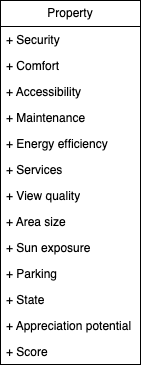
\includegraphics[width=0.3\linewidth]{property.png}
    \caption{Inferred attributes of a Property}
    \label{fig:property-attributes}
\end{figure}

\paragraph{}
\subsubsection{Rules}
In expert systems, rules are the core of decision-making and provide the mechanism to make inferences and conclusions.
For each attribute of a real estate Property we had several rules, describing how the value of that attribute influenced the final score of that Property. The systems took into account 13 different property attributes, however we had 14 different groups of rules. Group 14 describes the business rules for calculating the final score of the properties. In took into account the inferences of the previous rules and calculated the final score to be presented to the user.

Here are an excerpt of the business rules defined for our expert system:
\begin{table}[ht]
    \centering
    \begin{tabular}{c|c|c}
    \hline
    \textbf{ID} & \textbf{Category} & \textbf{Description} \\\hline
    1.1 & Security & If location crime rate is low then property crime rate is low \\\hline
    1.2 & Security & If location crime rate is medium then property crime rate is medium \\\hline
    1.3 & Security & If location crime rate is high then the property crime rate is high \\\hline
    1.4 & Security & If property crime rate is low and it has a security system then level of security is high  \\\hline
    1.5 & Security & If property crime rate is high and it doesn't have a security system then level of security is low \\\hline
    ... & ... & ... \\\hline
    6.1 & Services & If location has schools then the property has schools nearby \\\hline
    6.2 & Services & If location has public transports then the property has nearby public transports \\\hline
    6.3 & Services & If location has a hospital then the property has a nearby hospital \\\hline
    6.4 & Services & If location has supermarkets then the property has a nearby supermarket \\\hline
    6.5 & Services & If location has leisure areas then the property has nearby leisure areas \\\hline
    ... & ... & ... \\\hline
    14.1 & Scores & Calculates the security score \\\hline
    14.6 & Scores & Calculates the services score\\\hline
    14.7 & Scores & Calculates the connectivity score\\\hline
    14.14 & Scores & Calculates the final score of the property \\\hline
    \end{tabular}
    \caption{Excerpt of business rules defined from the expert's knowledge}
    \label{tab:rules}
\end{table}

\section{Results}

Our system despite being an early stage prototype still produced some promising results. To get a more realistic understanding of results we defined 3 different personas, with different demographics and different requirements for buying a house:

\begin{itemize}
    \item The retired expat - A recently retired 60+ person. Seeking a property in quiet place.
    \item The young remote worker - A young worker with a high income, usually single or partnered.
    \item The typical Portuguese family - a young couple with 1 or 2 of kids
\end{itemize}

The retired expat would be looking for a property in quiet location with low crime rate. Comfortable and security are of high priority for this persona. The appreciation potential and the accessibility are probably not the highest priorities for this persona.

The young remote worker would be most interested on a property that would allow them flexibility and comfort. Located in a city center so that services and near by and where social life can thrive. Appreciation potential is probably of high importance as well as services and sun exposure.

The typical Portuguese family has their kids life in top of mind. They need a property that can accommodate their busy life style but can still provide a safe and easy to manage environment for their children. Security is of high importance and maintenance cost need to be as low as possible. Schools and public transportation near the property are also of great importance.

We ran these 3 scenarios through our application and we were able to ascertain that the system does a fairly decent job in recommending properties given these very basic examples.

\subsubsection{Limitations and improvements} Of course with this system being an basic prototype there is still a lot of room for improvement. Starting by the availability of data, our system can only recommend properties for which it has the data in its knowledge base. So in order to obtain even better results one of the topics we'd have to improve would be the size, quality and diversification of our properties dataset.

Another aspect we've noticed could be improved was the computational cost of running this system. Given that we load all our dataset into memory so the engine can have access to it we face ourselves with a bottleneck in terms of performance. A strict physical limitation is encountered in the amount of memory where our system is running. A future improvement would be to move our dataset to more appropriate data infrastructure such as a Database Management System and implement a caching mechanism that would allow for easier access to the most searched for properties.

Another great initiative that we think would bring great value to our solution would be the addition of an Insights/Statistics component where it would track all the requests and results that the system received and generated, respectively. This would allow us to understand better how our system works and find hidden insights on where it would benefit the most to be improved.


\bibliographystyle{splncs04}
\bibliography{references}

\end{document}
